Cell line development (CLD) is a process of generating single cell-derived clones that produce high and consistent levels of target therapeutic protein (\cite{lonza}). Therapeutic proteins in this case are so-called recombinant proteins and they are widely used in biomedical research, the production of medication and for various therapeutic needs such as, for example, vaccines and monoclonal antibodies (mAbs) (\cite{Ohtake_2013}, \cite{Jefferis_2017}, \cite{Funaro_1996}). A recombinant protein, as defined by \cite{Barbeau_2018}, is a modified or manipulated protein encoded by a recombinant DNA. Recombinant DNA in turn consists of a plasmid, where the genes of the target protein of interest are cloned downstream of a promoter region. As soon as this plasmid is transfected to a host cell (for example some mammalian cells that are able to produce the protein), the host will start to express this protein of interest. Today there is a great need for the production of high volumes of good quality recombinant proteins, both in industrial as well as research contexts (\cite{Tihanyi_2020}). This is the reason why the goal of many research projects in recombinant protein production is to improve expression efficiency and create high-throughput systems to improve the CLD processes (\cite{Tihanyi_2020}).

%\cite[see]{IWNLP} \supercite{iqbal2007underwater}

One of the most popular host cells used in CLD and in this thesis specifically are chinese hamster ovary (CHO) cells [cite Castan 2018]. Although different cells can be used as hosts, such as bacterial, plant-based or yeast cells, mammalian cells remain the most popular choice [cite Beckman]. The reason behind this popularity resides in the fact that they can produce a diverse range of correctly folded proteins and most importantly they have high protein production rates. The productivity rate is measured in titre of produced protein, and CHO cells can reach 0.1 - 1 g/L in batch and 1 - 10 g/L in fed-batch [TODO add reference] cultures [cite Tihanyi 2020]. Mostly all of the mAbs are produced using CHO cells [cite Lalonde 2017]. Companies mostly use the same host cell line for all their productions because already checked and qualified cells simplify the road to the clinic [cite Tihanyi 2020]. This is why current research has a wide applicability.

However, there is a downside to using CHO as host cells - they are infamously unstable. As rapidly growing immortal cells CHO are also genomically unstable and extremely heterogeneous which usually leads to the main issue: production instability. The problem of choosing stable and high-production clones that simultaneously will be able to express protein qualitatively and quantifiably over time is essentially the main goal of current research. The challenge in manufacturing here is the time and the cost of production. Currently, a lot of research attention is dedicated to the reduction of both factors, as well as the development of techniques of high-throughput clone screening and characterization [cite Tihanyi 2020]. The latter is of interest for this thesis. With great amounts of data collected over time and the development of computational modelling and statistical analysis it is now possible to carry out the analysis \textit{in silico}, meaning computationally without interfering with the cells instead of the usual \textit{in vitro} analysis.

\paragraph{CLD steps}
\begin{figure}[H]
	\begin{center}
		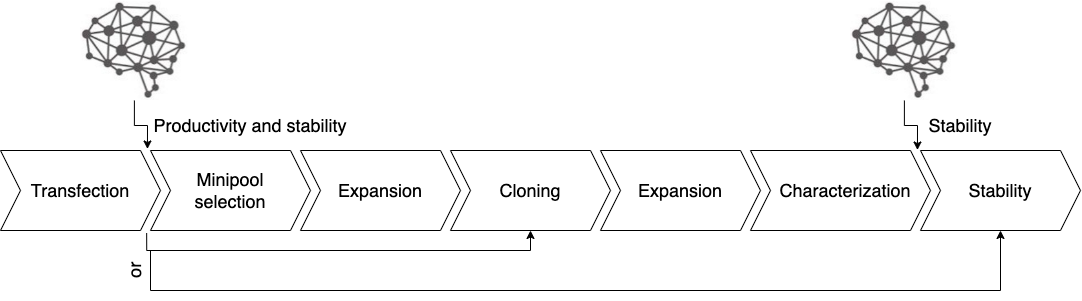
\includegraphics[width=0.8\linewidth]{bilder/CLD.png}
		\caption{CLD process steps}\label{fig:cls-steps}
	\end{center}
\end{figure}

The first step of CLD is called transfection - the introduction of the gene of interest (GOI or a DNA vector or alternatively an expression vector) into CHO cells. There are two main problems with this step: firstly, transfection mostly results in a vector being inserted into a random site within the host cell genome and secondly, it generally has low efficiency of integration [cite Tihanyi]. It is important to transfect a GOI into the optimal site of the genome to secure high protein expression over time during protein production. Practically however, GOI is transfected into a random location of genome. In cases where the gene was transfected into an inactive site of genome (essentially the majority of genome is transcriptionally inactive), the cell will likely be unable to express the gene [cite Castan, Hong 2018].

The second step of the process is the selection of cell minipools that have successful and stable gene integrations for further expansion and cloning. The reason for not all of them being suitable is that during the transfection step, only 80\% of the cells will receive a GOI vector [cite Castan]. Only a small percentage of these cells actually integrate a vector into the genome and, as mentioned above, only a fraction of those are able to express the protein stably [a better reference needed Shin 2020]. After the best minipools are selected, they will be expanded.

The third step in CLD is to clone the cells. The selected stable pools of cells are phenotypically and genetically diverse. This means that they have different growth rates, metabolic profiles, and so forth. This is not ideal for industrial production - all the cells used for protein production should be derived from the same clone [cite [25] from Castan]. 

Once the cells are cloned, phenotypical and genetical heterogeneity is reduced, the next step is to characterize the cells for their expression of the GOI. One has to estimate the clones' productivity and stability. Such observations may take up to 90 days (usually the checks are made on the $30^{\text{th}}$, $60^{\text{th}}$ and $90^{\text{th}}$ days). If the clones remain stable after this time and are able to express enough of the protein, then they are suitable for further production. However, this last step costs a lot of time and maintenance costs for feeding and analysing the cells. Predicting productivity and stability of the cells in earlier stages would reduce this time significantly or even allow to avoid this process entirely. 